%%%%%%%%%%%%%%%%%%%%%%%%%%%%%%%%%%%%%%%%%%%%%%%%%%%%%%%%%%%%%%%%%%%%%%%%%%%%%%%
%                         UNIDAD 1: COMUNICACIÓN SERIE                        %
%%%%%%%%%%%%%%%%%%%%%%%%%%%%%%%%%%%%%%%%%%%%%%%%%%%%%%%%%%%%%%%%%%%%%%%%%%%%%%%

\chapter{Unidad 1: Comunicación Serie}

\section{¿Por qué comunicamos dispositivos?}

En cualquier sistema industrial moderno, los componentes necesitan intercambiar información: un sensor debe enviar una medida a un controlador, un PLC debe ordenar un movimiento a un motor, o un ordenador debe supervisar el estado de toda una planta. Esta necesidad de compartir datos entre dispositivos electrónicos es el origen de las comunicaciones digitales.

A lo largo de la historia, los ingenieros han buscado formas cada vez más eficientes de transmitir información. Desde el telégrafo de Samuel Morse (1844), que enviaba puntos y rayas por un único cable, hasta las redes industriales actuales que mueven gigabytes por segundo, el principio fundamental es el mismo: codificar información, transportarla por un medio físico y decodificarla en el destino.

\begin{figure}[H]
\centering
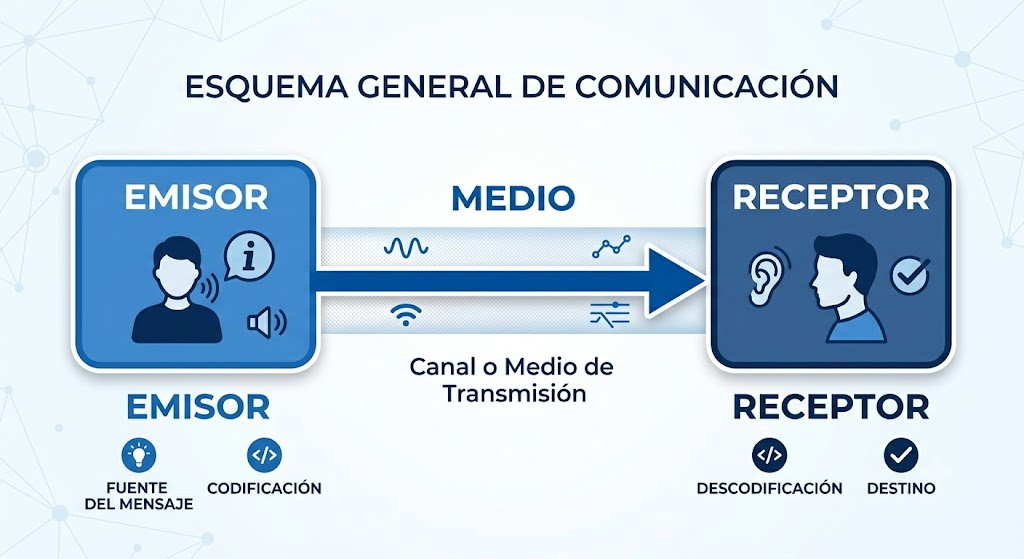
\includegraphics[width=0.8\textwidth]{assets/cap1/1.1.jpeg}
\caption{Modelo conceptual de cualquier comunicación: origen, medio y destino}
\label{fig:modelo-comunicacion}
\end{figure}

Hoy en día, la decisión más básica que enfrenta un diseñador de sistemas embebidos es: ¿transmito los datos en paralelo o en serie?


\section{Transmisión paralela vs. transmisión en serie}

\subsection{Transferencia en paralelo}

En una transmisión paralela, todos los bits de una palabra de datos se envían simultáneamente por múltiples líneas independientes. Por ejemplo, para transmitir un byte completo (8 bits), se necesitan 8 cables de datos, más las líneas de control y tierra.

\begin{definicion}
La \textbf{transferencia de datos en paralelo} es un método de comunicación en el que todos los bits de una palabra de datos se transmiten simultáneamente a través de múltiples canales físicos independientes.
\end{definicion}

Las ventajas parecen claras: es rápida, ya que un byte completo llega en un solo ciclo. Sin embargo, esta aparente ventaja desaparece cuando se analizan los problemas físicos:

\begin{itemize}
    \item \textbf{Coste hardware elevado}: cada bit requiere su propio conductor, conector y circuito de E/S.
    \item \textbf{Diafonía}: a alta velocidad, las señales eléctricas de un cable se acoplan a los adyacentes por efecto capacitivo e inductivo, generando ruido.
    \item \textbf{Sesgo de tiempo (skew)}: los cables no tienen exactamente la misma longitud ni impedancia, por lo que los bits llegan ligeramente desfasados. A velocidades altas, este desfase puede causar errores.
    \item \textbf{Limitación de distancia}: a frecuencias de decenas de Mb/s, los buses paralelos solo funcionan en trayectos de pocos centímetros. A Gb/s, apenas unos milímetros dentro de un chip.
\end{itemize}

\begin{figure}[H]
\centering
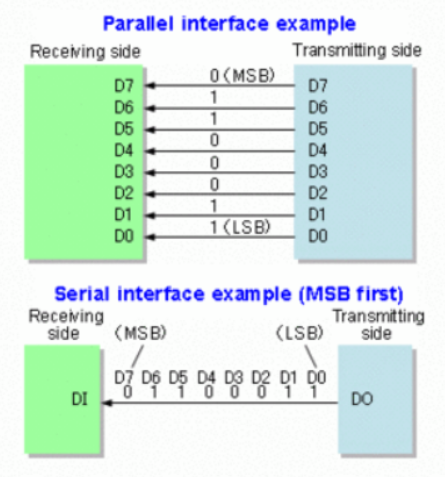
\includegraphics[width=0.8\textwidth]{assets/cap1/1.2.png}
\caption{Comparación visual: transmisión paralela (8 líneas) vs. transmisión en serie (1 línea)}
\label{fig:paralelo-vs-serie}
\end{figure}

\subsection{Transferencia en serie}

En una transmisión en serie, los bits se envían uno tras otro por una única línea de datos (más tierra). El byte completo tarda más tiempo en llegar, pero el hardware es mucho más sencillo.

\begin{definicion}[formal de transferencia en serie]
La \textbf{transferencia de datos en serie} es un método de comunicación en el que los bits de una palabra se transmiten secuencialmente, uno tras otro, a través de un único canal físico.
\end{definicion}

Las ventajas de la transmisión en serie son:
\begin{itemize}
    \item \textbf{Menor coste}: un solo cable de datos, conectores más pequeños y menos pines en los circuitos integrados.
    \item \textbf{Mayor inmunidad al ruido}: con técnicas de transmisión diferencial (ver sección \ref{sec:balanceado}), el ruido se cancela.
    \item \textbf{Distancias mayores}: algunas interfaces serie alcanzan cientos de metros (RS-485) o kilómetros (fibra óptica).
    \item \textbf{Velocidades elevadas}: aunque los bits llegan de uno en uno, las frecuencias de reloj pueden ser muy altas (Gb/s en USB, SATA, fibra óptica).
\end{itemize}

La principal desventaja es temporal: transmitir un byte en serie tarda más que en paralelo. Sin embargo, en la mayoría de aplicaciones industriales y de comunicaciones, esta diferencia es irrelevante frente a los beneficios de simplicidad y fiabilidad.

\begin{table}[htbp]
\centering
\small
\caption{Comparativa: transmisión paralela vs. en serie}
\begin{tabularx}{\textwidth}{@{}lXX@{}}
\toprule
\textbf{Característica} & \textbf{Paralelo} & \textbf{Serie} \\
\midrule
Número de líneas de datos & N (una por bit) & 1 \\
Velocidad por transferencia & Alta (1 byte/ciclo) & Más lenta (1 bit/ciclo) \\
Coste hardware & Elevado (muchos pines, cables) & Bajo (pocos pines, cables) \\
Diafonía & Problema grave a alta velocidad & Prácticamente nulo \\
Distancia máxima & Centímetros a metros & Metros a kilómetros \\
Aplicaciones típicas & Buses internos de PCB, RAM & USB, Ethernet, UART, SATA \\
\bottomrule
\end{tabularx}
\end{table}


\subsection{Principales interfaces de comunicación serie}

A continuación se resumen las interfaces serie más relevantes en el ámbito de la electrónica, la informática industrial y las redes de comunicaciones:

\begin{table}[H]
\centering
\footnotesize
\caption{Principales tipos de interfaces seriales}
\begin{tabularx}{\textwidth}{@{}>{\raggedright\arraybackslash}p{2.5cm}>{\raggedright\arraybackslash}X>{\raggedright\arraybackslash}p{3.5cm}@{}}
\toprule
\textbf{Interfaz} & \textbf{Descripción} & \textbf{Aplicación típica} \\
\midrule
SPI & Comunicación síncrona de alta velocidad. Maestro y múltiples esclavos. & Memoria flash, pantallas, tarjetas SD \\
I2C & Comunicación bidireccional con dos líneas (datos y reloj). & Sensores, EEPROM, displays \\
UART & Protocolo asíncrono básico, común en sistemas embebidos. & Debug, GPS, módems, Bluetooth \\
RS-232 / RS-422 / RS-485 & Estándares industriales. RS-232 en módems; RS-485 en automatización. & PLCs, módems, redes industriales \\
USB & Interfaz estándar moderna para periféricos de computadora. & Teclados, discos, cámaras \\
SATA & Conexión de discos duros internos. & SSD, HDD \\
CAN & Red para automoción y automatización industrial. & Automóviles, maquinaria, buses \\
1-Wire & Interfaz de bajo costo para pocos componentes. & Sensores de temperatura, iButton \\
\bottomrule
\end{tabularx}
\end{table}


\section{Tipos de codificación en comunicaciones serie}

Antes de que los bits viajen por el medio físico, deben convertirse en señales eléctricas (o luminosas) que el receptor pueda interpretar. El proceso de convertir un bit lógico (0 o 1) en una forma de onda física se denomina \textbf{codificación de línea}. La elección de la codificación afecta directamente a la inmunidad al ruido, la capacidad de recuperación de reloj y la eficiencia espectral del canal.

\subsection{NRZ (Non-Return-to-Zero)}

En la codificación NRZ, el nivel de tensión se mantiene constante durante todo el periodo de bit: un nivel alto representa un ``1'' y un nivel bajo representa un ``0''. Es el método más sencillo, pero presenta dos inconvenientes principales: no garantiza transiciones cuando se transmiten largas secuencias del mismo bit, lo que dificulta la recuperación de reloj, y tiene una componente continua (DC) que no es adecuada para algunos medios acoplados con transformador.

\begin{figure}[H]
\centering
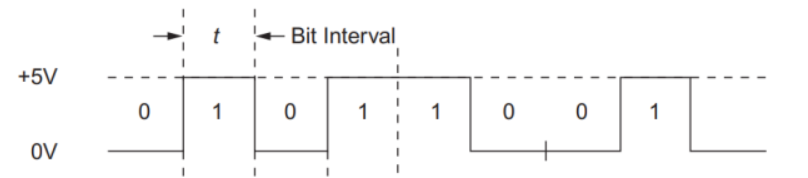
\includegraphics[width=0.8\textwidth]{assets/cap1/1.3.png}
\caption{Ejemplo de codificación NRZ para una secuencia de bits}
\label{fig:codificacion-nrz}
\end{figure}

\subsection{NRZ bipolar}

En la codificación NRZ bipolar, los bits ``1'' y ``0'' se representan mediante dos niveles de tensión de polaridad opuesta (por ejemplo, $+$V para ``1'' y $-$V para ``0''). A diferencia del NRZ unipolar, esta variante no presenta componente continua y mejora la inmunidad al ruido, ya que el receptor puede detectar la información midiendo la polaridad de la señal.

\begin{figure}[H]
\centering
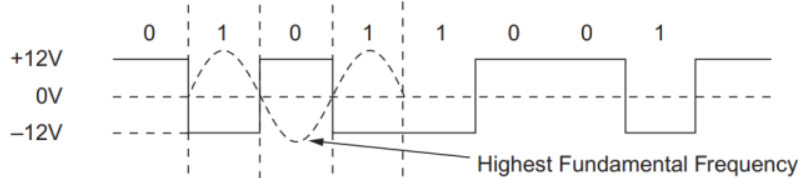
\includegraphics[width=0.8\textwidth]{assets/cap1/1.4.png}
\caption{Ejemplo de codificación NRZ bipolar}
\label{fig:codificacion-nrz-bipolar}
\end{figure}

\subsection{NRZ invertida (NRZ-I)}

En la codificación NRZ invertida (NRZ-I), la señal \textbf{no cambia} para un ``0'' y \textbf{invierte} su polaridad para un ``1''. De esta forma, una secuencia de unos produce transiciones continuas, mientras que una secuencia de ceros mantiene el nivel. NRZ-I se utiliza en interfaces como USB (junto con bit stuffing) para garantizar suficientes transiciones y permitir la recuperación de reloj.

\begin{figure}[H]
\centering
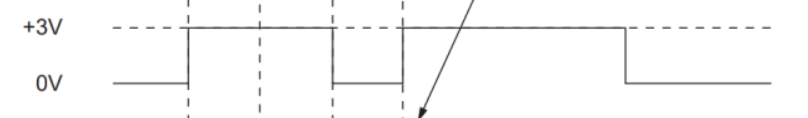
\includegraphics[width=0.8\textwidth]{assets/cap1/1.5.png}
\caption{Ejemplo de codificación NRZ invertida (NRZ-I)}
\label{fig:codificacion-nrzi}
\end{figure}

\subsection{RZ (Return-to-Zero)}

En RZ, la señal vuelve a cero (o al nivel de referencia) en la \textbf{mitad} del periodo de bit, independientemente del valor transmitido. Por ejemplo, en RZ unipolar, un ``1'' se representa como un pulso positivo seguido de un retorno a cero, mientras que un ``0'' se mantiene en nivel cero. Aunque simplifica la sincronización, consume más ancho de banda que NRZ.

\begin{figure}[H]
\centering
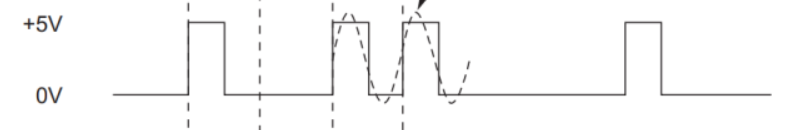
\includegraphics[width=0.8\textwidth]{assets/cap1/1.6.png}
\caption{Ejemplo de codificación RZ (Return-to-Zero)}
\label{fig:codificacion-rz}
\end{figure}

\subsection{RZ bipolar}

En la variante RZ bipolar, un ``1'' se representa como un pulso positivo seguido de retorno a cero, y un ``0'' como un pulso negativo seguido de retorno a cero. Requiere tres niveles de tensión (positivo, cero y negativo), lo que complica los circuitos, pero proporciona una referencia de nivel clara y permite detectar la pérdida de señal.

\begin{figure}[H]
\centering
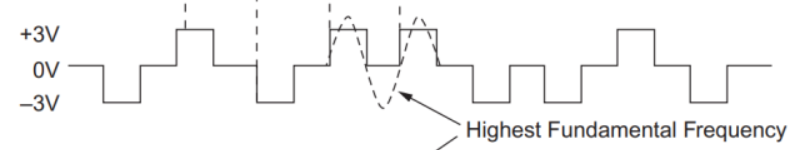
\includegraphics[width=0.8\textwidth]{assets/cap1/1.7.png}
\caption{Ejemplo de codificación RZ bipolar}
\label{fig:codificacion-rz-bipolar}
\end{figure}

\subsection{Manchester}

La codificación Manchester resuelve el problema de la recuperación de reloj generando \textbf{siempre una transición en el centro de cada bit}: una transición de bajo a alto representa un ``1'', y de alto a bajo representa un ``0''. Garantiza una transición por bit, lo que facilita enormemente la sincronización, pero duplica el ancho de banda necesario porque la frecuencia de la señal es el doble de la tasa de bits. Se empleó históricamente en Ethernet 10BASE-T.

\begin{figure}[H]
\centering
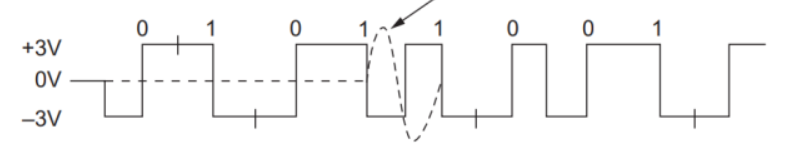
\includegraphics[width=0.8\textwidth]{assets/cap1/1.8.png}
\caption{Ejemplo de codificación Manchester}
\label{fig:codificacion-manchester}
\end{figure}

\begin{table}[htbp]
\centering
\small
\caption{Resumen comparativo de codificaciones de línea}
\begin{tabularx}{\textwidth}{@{}lXXX@{}}
\toprule
\textbf{Codificación} & \textbf{Transiciones} & \textbf{Componente DC} & \textbf{Uso típico} \\
\midrule
NRZ & No garantizadas & Sí & UART, SPI (interno) \\
NRZ bipolar & En cada bit (cambio de polaridad) & No & Telecomunicaciones \\
NRZ-I (invertida) & Sólo en unos (con bit stuffing) & Sí & USB \\
RZ (unipolar) & Garantizadas (retorno a cero) & Sí & Canales de fibra óptica antiguos \\
RZ bipolar & Garantizadas (tres niveles) & No & Telecomunicaciones, satélite \\
Manchester & Garantizadas (1/bit) & No & Ethernet 10BASE-T \\
\bottomrule
\end{tabularx}
\end{table}


\section{Conceptos fundamentales de las comunicaciones serie}
\label{sec:fundamentos}

\subsection{Topologías de conexión}

La topología describe cómo se conectan físicamente los nodos de una red:

\begin{itemize}
    \item \textbf{Punto a punto (peer-to-peer)}: la conexión más simple, con solo dos nodos. Ejemplo: un PC conectado a una impresora, o un microcontrolador a un sensor.
    \item \textbf{Bus}: todos los nodos comparten un mismo medio de transmisión. Ejemplo: RS-485, CAN bus.
    \item \textbf{Estrella}: todos los nodos se conectan a un nodo central. Ejemplo: Ethernet con switch, USB con hub.
    \item \textbf{Anillo}: cada nodo se conecta a dos vecinos, formando un círculo. Ejemplo: redes industriales antiguas, anillos ópticos.
\end{itemize}

\begin{figure}[H]
\centering
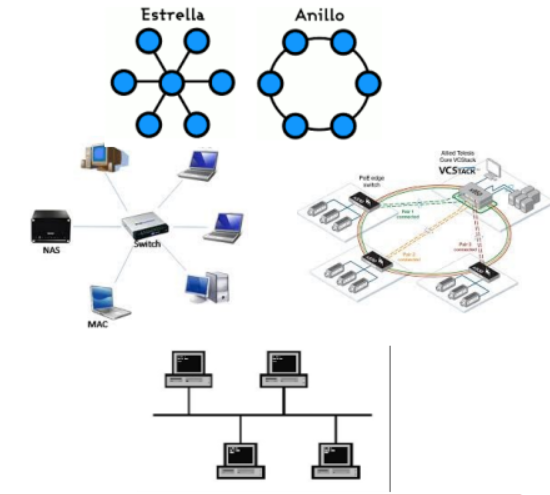
\includegraphics[width=0.8\textwidth]{assets/cap1/1.9.png}
\caption{Las cuatro topologías básicas en comunicaciones serie}
\label{fig:topologias}
\end{figure}

\subsection{Configuraciones balanceadas vs. no balanceadas}
\label{sec:balanceado}

Esta distinción es fundamental para entender la inmunidad al ruido de una comunicación.

\subsubsection{Conexión no balanceada (single-ended)}

En una conexión no balanceada, la señal se transmite por un único conductor y se toma como referencia la tierra (GND). El voltaje de la señal se mide respecto a tierra.

\begin{definicion}[formal de conexión no balanceada]
Una conexión \textbf{no balanceada} (o desbalanceada) es aquella en la que el voltaje de señal se referencia a un punto de tierra común, utilizando un único conductor para transportar la información.
\end{definicion}

Es sencilla y económica, pero tiene un problema grave: cualquier ruido inducido en el cable o diferencia de potencial entre las tierras de los dos dispositivos se suma directamente a la señal, pudiendo causar errores.

\subsubsection{Conexión balanceada (diferencial)}

En una conexión balanceada, la señal se transmite por dos conductores, ninguno de los cuales está conectado a tierra. Los voltajes en ambos conductores son de polaridad opuesta respecto a tierra. El receptor no mide el voltaje respecto a tierra, sino la \textbf{diferencia} entre ambos conductores.

\begin{definicion}[formal de conexión balanceada]
Una conexión \textbf{balanceada} (o diferencial) es aquella en la que la señal se transmite mediante dos conductores con voltajes de polaridad opuesta, y el receptor recupera la información calculando la diferencia entre ambos voltajes.
\end{definicion}

\textbf{¿Por qué cancela el ruido?} Si un ruido externo se acopla a la línea, afecta por igual a los dos conductores. Como el receptor resta los voltajes, la componente de ruido común ($V_{ruido} - V_{ruido} = 0$) desaparece. Esto se conoce como \textbf{rechazo al modo común (CMRR)}.

\begin{figure}[H]
\centering
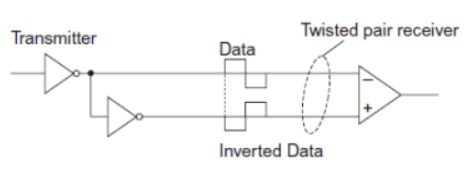
\includegraphics[width=0.8\textwidth]{assets/cap1/1.10.png}
\caption{Cancelación del ruido en una conexión balanceada (diferencial)}
\label{fig:balanceada}
\end{figure}

\subsection{Medios de transmisión físicos}

Los datos en serie pueden viajar por diferentes medios. Los más comunes son:

\subsubsection{Líneas en placa de circuito impreso (PCB)}

Son las trazas de cobre que conectan chips dentro de una misma placa. Son cortas (centímetros) y pueden ser desbalanceadas (traza + tierra) o balanceadas (dos trazas paralelas). Su uso se limita a comunicaciones internas de alta velocidad entre circuitos integrados vecinos.

\subsubsection{Cable coaxial}

Un conductor central rodeado por una malla metálica (blindaje) y una cubierta exterior. Es una línea desbalanceada con impedancia característica típica de $50\,\Omega$. Aunque la atenuación es considerable, puede transportar señales de varios Gb/s en distancias cortas. Hoy se usa principalmente en RF y en algunas redes de comunicaciones.

\begin{figure}[H]
\centering
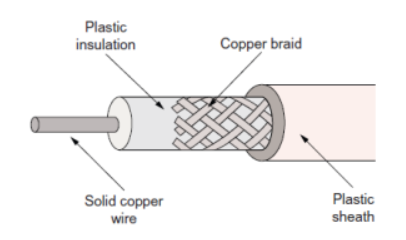
\includegraphics[width=0.8\textwidth]{assets/cap1/1.11.png}
\caption{Ejemplo de cable coaxial}
\label{fig:cable-coaxial}
\end{figure}

\subsubsection{Par trenzado (UTP/STP)}

Dos cables aislados retorcidos entre sí, sin blindaje (UTP) o con blindaje (STP). Es el medio más utilizado en redes modernas:
\begin{itemize}
    \item El retorcido reduce la diafonía entre pares adyacentes.
    \item El blindaje (en STP) protege en entornos industriales ruidosos.
    \item Ejemplos: cableado telefónico, Ethernet CAT5/CAT6.
\end{itemize}

\begin{figure}[H]
\centering
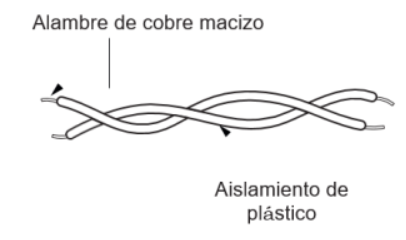
\includegraphics[width=0.8\textwidth]{assets/cap1/1.12.png}
\caption{Ejemplo de par trenzado (UTP/STP)}
\label{fig:par-trenzado}
\end{figure}

\subsubsection{Fibra óptica}

Un núcleo de vidrio o plástico rodeado de revestimiento y cubierta. Los datos se convierten en pulsos de luz infrarroja generados por LEDs o láseres. En el receptor, un fotodiodo (PIN o avalancha) convierte la luz de nuevo en señal eléctrica.

Sus ventajas son excepcionales:
\begin{itemize}
    \item Velocidades superiores a 100\,Gb/s.
    \item Inmunidad total al ruido eléctrico y a la diafonía.
    \item Distancias de kilómetros sin regeneración.
\end{itemize}

\begin{figure}[H]
\centering
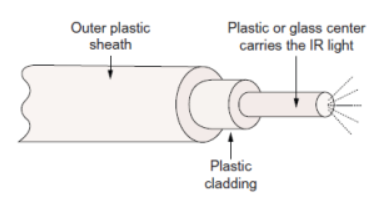
\includegraphics[width=0.8\textwidth]{assets/cap1/1.13.png}
\caption{Ejemplo de fibra óptica}
\label{fig:fibra-optica}
\end{figure}


\section{El reloj: cómo se sincronizan emisor y receptor}
\label{sec:reloj}

En cualquier comunicación digital, el receptor debe saber \textbf{cuándo} leer cada bit. Si muestrea demasiado pronto o demasiado tarde, leerá un valor incorrecto. La sincronización se resuelve mediante una señal de reloj. En comunicaciones serie existen tres estrategias fundamentales.

\subsection{Transmisión asíncrona: relojes independientes}

Cada dispositivo tiene su propio reloj interno. Los relojes no están sincronizados, pero deben coincidir aproximadamente en frecuencia. Para que el receptor sepa cuándo empieza un nuevo dato, el transmisor añade un \textbf{bit de inicio} (start bit) antes de los datos propiamente dichos. Al detectar esta transición, el receptor recalibra su muestreo para el byte siguiente.

\begin{figure}[H]
\centering
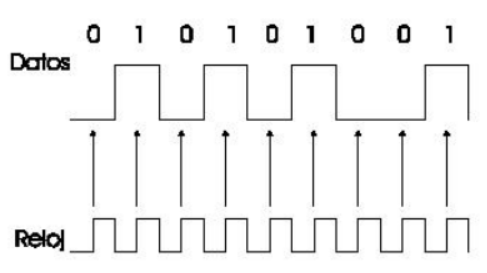
\includegraphics[width=0.8\textwidth]{assets/cap1/1.14.png}
\caption{Formato típico de una transmisión asíncrona byte a byte (ejemplo UART)}
\label{fig:trama-asincrona}
\end{figure}

\textbf{Ventaja}: solo se necesita una línea de datos (más tierra). 
\textbf{Limitación}: las frecuencias de reloj deben ser muy similares, y se desperdicia algo de tiempo en los bits de sincronización de cada byte.

\subsection{Transmisión síncrona: reloj en línea separada}

El transmisor envía una señal de reloj por un cable adicional, junto con la línea de datos. El receptor muestrea los datos exactamente en los flancos de este reloj externo.

\textbf{Ventaja}: sincronización perfecta, sin margen de error por desajuste de relojes.
\textbf{Desventaja}: requiere una línea adicional (dos líneas de señal + tierra), lo que encarece el cableado.

\subsection{Recuperación de reloj desde los datos (CDR)}

En las comunicaciones más rápidas, no hay línea de reloj separada ni bits de inicio/parada. El receptor extrae el reloj directamente de las transiciones de la propia señal de datos. Para que esto funcione, los datos deben codificarse de forma que haya suficientes transiciones (0→1 y 1→0), evitando secuencias largas del mismo nivel.

\begin{definicion}[formal de CDR]
La técnica de \textbf{reloj y recuperación de datos (CDR, Clock and Data Recovery)} consiste en reconstruir la señal de reloj a partir de las transiciones de la propia señal de datos recibida, permitiendo la sincronización sin necesidad de una línea de reloj separada.
\end{definicion}

Este método se usa en interfaces de alta velocidad como USB 3.0, SATA, PCIe y Ethernet de fibra óptica.

\begin{table}[htbp]
\centering
\small
\caption{Los tres métodos de sincronización en comunicaciones serie}
\begin{tabularx}{\textwidth}{@{}lXX@{}}
\toprule
\textbf{Método} & \textbf{Característica} & \textbf{Ejemplo} \\
\midrule
Asíncrona & Relojes independientes, bits de inicio/parada & UART, RS-232 \\
Síncrona (reloj separado) & Línea de reloj adicional, perfecta sincronización & SPI, I2C \\
CDR & Reloj extraído de los datos, codificación especial & USB 3.0, SATA, Ethernet \\
\bottomrule
\end{tabularx}
\end{table}


\section{Formatos de trama y protocolos}

Un \textbf{protocolo} es el conjunto de reglas que definen cómo se comunican dos dispositivos: el formato de los datos, el orden de los bits, la detección de errores, el control de flujo, etc.

La mayoría de los datos se envían en bloques estructurados llamados \textbf{tramas} o \textbf{frames}. Aunque cada protocolo tiene su propio formato, la estructura general sigue un patrón común:

\begin{enumerate}
    \item \textbf{Delimitador de inicio}: una secuencia especial de bits que indica ``aquí empieza una trama''.
    \item \textbf{Dirección}: identifica el nodo destino (y a veces el origen).
    \item \textbf{Datos}: el contenido propiamente dicho, normalmente un bloque de bytes.
    \item \textbf{Código de control de errores}: un valor calculado a partir de los datos (paridad, CRC, BCC) para detectar o corregir errores.
    \item \textbf{Delimitador de fin}: señala el final de la trama.
\end{enumerate}

\begin{figure}[H]
\centering
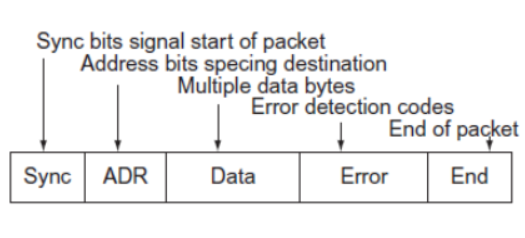
\includegraphics[width=0.8\textwidth]{assets/cap1/1.15.png}
\caption{Estructura genérica de una trama de datos en comunicaciones serie}
\label{fig:trama-generica}
\end{figure}

\subsection{Transmisión asíncrona vs. síncrona de tramas}

\begin{itemize}
    \item \textbf{Asíncrona}: cada byte se envía de forma independiente con sus propios bits de inicio y parada. No hay una estructura de trama compleja; se transmiten bytes sueltos.
    \item \textbf{Síncrona}: los datos se agrupan en tramas largas. No hay bits de inicio/parada por cada byte; en su lugar, la trama comienza con un delimitador especial y el receptor usa CDR o una línea de reloj para muestrear continuamente.
\end{itemize}


\section{Detección y corrección de errores}

El ruido electromagnético, las interferencias y las imperfecciones del medio pueden alterar los bits durante la transmisión. Por eso, los protocolos serie incorporan mecanismos para detectar o incluso corregir errores.

\subsection{Bit de paridad}

Es el método más sencillo. Consiste en añadir un bit extra a cada byte transmitido, de forma que el número total de bits a 1 sea par (paridad par) o impar (paridad impar).

\begin{definicion}[formal del bit de paridad]
El \textbf{bit de paridad} es un bit adicional que se añade a una palabra de datos para que el número total de bits con valor 1 sea par (paridad par) o impar (paridad impar). El receptor recuenta los bits y compara con el bit de paridad recibido; si hay discrepancia, se detecta un error.
\end{definicion}

\textbf{Limitación}: solo detecta errores cuando cambia un número impar de bits. Si dos bits se invierten simultáneamente, la paridad no lo detecta. Además, no indica qué bit está mal, solo que ha ocurrido un error.

\subsection{Código de verificación de bloques (BCC / BCS)}

En lugar de verificar byte a byte, se puede calcular un código de verificación para un bloque completo de datos. Un método sencillo es el \textbf{BCC (Block Check Character)}: se suman (o se hace XOR) todos los bytes del bloque, y el resultado final se envía como un carácter de verificación al final de la trama. El receptor repite el cálculo y compara.

Este método permite detectar errores en múltiples bits del bloque, pero no identificar la posición exacta del error.

\subsection{Verificación de redundancia cíclica (CRC)}

El CRC es el método más robusto de detección de errores en comunicaciones serie industriales. Se trata los bits de datos como una secuencia binaria y se divide por un polinomio generador predefinido mediante aritmética modular. El resto de esta división (el CRC) se adjunta a la trama y se verifica en el receptor.

El CRC detecta eficazmente las \textbf{ráfagas de errores} (varios bits consecutivos alterados), siempre que la longitud de la ráfaga no supere el grado del polinomio generador.

\begin{table}[htbp]
\centering
\small
\caption{Comparativa de métodos de detección de errores}
\begin{tabularx}{\textwidth}{@{}lXXX@{}}
\toprule
\textbf{Método} & \textbf{Complejidad} & \textbf{Eficacia} & \textbf{Uso típico} \\
\midrule
Bit de paridad & Muy baja & Detecta 1 bit impar & UART, RS-232 \\
BCC/BCS & Baja & Detecta errores simples & Protocolos antiguos \\
CRC & Media & Detecta ráfagas de errores & Ethernet, CAN, USB, industrial \\
\bottomrule
\end{tabularx}
\end{table}


\subsection{Corrección de errores de reenvío (FEC)}

Además de detectar errores, algunos protocolos de comunicación serie son capaces de \textbf{corregirlos} sin necesidad de retransmisión. La técnica se conoce como \textbf{Forward Error Correction (FEC)} o corrección de errores de reenvío.

Los métodos FEC añaden información redundante calculada a partir de los datos originales. Si la señal recibida se deteriora por ruido o interferencias, el receptor utiliza esa redundancia para reconstruir los bits erróneos. Esto mejora la fiabilidad de la transmisión y reduce la tasa de errores de bits (BER).

Una ventaja notable de los sistemas FEC es que, en presencia de ruido, actúan como si el sistema produjera \textbf{ganancia de codificación}. Esta ganancia compensa el ruido en el canal y permite alcanzar velocidades de datos más altas sin aumentar la potencia de transmisión. Por ello, el FEC es fundamental en interfaces seriales de alta velocidad, comunicaciones por satélite y sistemas de almacenamiento masivo.




\section{Métodos de acceso al medio}

Cuando más de dos dispositivos comparten un mismo medio de transmisión, es necesario establecer un mecanismo que determine quién puede transmitir y cuándo. Estos mecanismos se denominan \textbf{métodos de acceso al medio} y son la base de cualquier red multipunto o bus compartido.

\subsection{Maestro--Esclavo}

En un sistema de acceso maestro--esclavo, un único dispositivo \textbf{maestro} controla dos o más dispositivos \textbf{esclavos}. El maestro decide qué esclavo debe transmitir o recibir en cada momento, evitando colisiones en el medio compartido. Los protocolos de interfaz utilizan comandos específicos para instruir a los esclavos, y todas las operaciones están determinadas por el maestro.

Una técnica común es el \textbf{sondeo} (polling): el maestro consulta a cada esclavo en secuencia, enviando o recibiendo datos según sea necesario. Si un esclavo no tiene información, responde con una indicación de ``no hay datos'' y el maestro pasa al siguiente. Este método es sencillo, determinista y ampliamente utilizado en buses industriales como SPI y I2C.

\begin{figure}[H]
\centering
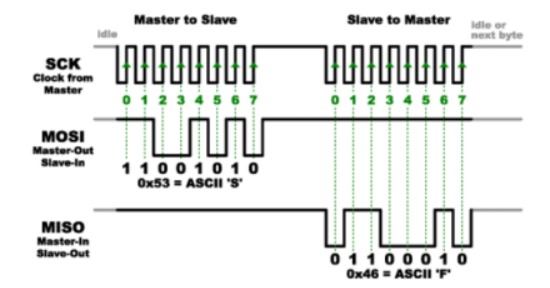
\includegraphics[width=0.8\textwidth]{assets/cap1/1.16.png}
\caption{Topología maestro--esclavo en un bus compartido}
\label{fig:maestro-esclavo}
\end{figure}

\subsection{CSMA (Carrier Sense Multiple Access)}

El \textbf{acceso múltiple por detección de portadora (CSMA)} es un sistema en el que todos los nodos de un bus ``escuchan'' el medio antes de transmitir. Si detectan que ya hay datos en tránsito (un ``portador'' presente), esperan para evitar colisiones.

La mayoría de los sistemas CSMA incorporan también \textbf{detección de colisiones (CD)}. Si dos dispositivos transmiten simultáneamente, sus señales se mezclan y generan errores. CSMA/CD detecta la colisión, hace que ambos nodos dejen de transmitir y esperen un tiempo aleatorio antes de reintentarlo. Aunque este método maneja automáticamente la contención, la competencia por el bus reduce el rendimiento global y aumenta la latencia, especialmente cuando hay muchos nodos activos.

\begin{figure}[H]
\centering
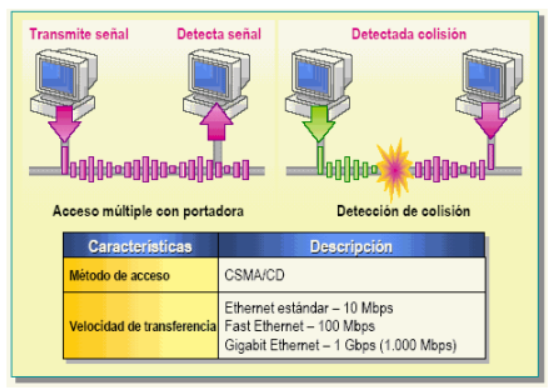
\includegraphics[width=0.8\textwidth]{assets/cap1/1.17.png}
\caption{Ejemplo de CSMA/CD con detección de colisión y retransmisión}
\label{fig:csma-cd}
\end{figure}

\subsection{TDMA (Time Division Multiple Access)}

El \textbf{acceso múltiple por división de tiempo (TDMA)} asigna a cada nodo una \textbf{franja horaria} (time slot) dentro de un ciclo periódico. El sistema define una unidad de tiempo para un ciclo completo y la divide en intervalos, uno para cada nodo del medio compartido. Cuando un dispositivo necesita transmitir, espera su intervalo asignado y envía los datos durante ese tiempo.

Las franjas horarias suelen ser de una palabra o un byte, aunque pueden ser más largas según el protocolo. Aunque la velocidad de transmisión instantánea de cada nodo se ve limitada por este método, en la mayoría de sistemas industriales la velocidad global es tan alta que el tiempo añadido no supone una desventaja significativa. TDMA es muy común en redes inalámbricas, sistemas GSM y buses industriales deterministas.

\begin{figure}[H]
\centering
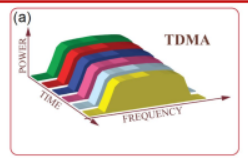
\includegraphics[width=0.8\textwidth]{assets/cap1/1.18.png}
\caption{Ejemplo de ciclo TDMA con cuatro nodos}
\label{fig:tdma}
\end{figure}

\subsection{Dúplex (Duplexing)}

El término \textbf{dúplex} se refiere a la direccionalidad de las comunicaciones entre dos dispositivos:

\begin{itemize}
    \item \textbf{Simplex}: comunicación unidireccional. Solo un dispositivo transmite y el otro recibe; no hay respuesta. Ejemplo: un sensor que envía lecturas continuamente a un display.
    \item \textbf{Semidúplex (half-duplex)}: ambos dispositivos pueden transmitir y recibir, pero \textbf{no simultáneamente}. Comparten un único canal y alternan turnos. Ejemplo: walkie-talkies, RS-485 en modo semidúplex.
    \item \textbf{Dúplex completo (full-duplex)}: transmisión y recepción \textbf{simultáneas}. En sistemas cableados se requieren dos canales físicos (uno para cada dirección). Ejemplo: UART, RS-232, Ethernet.
\end{itemize}

En sistemas inalámbricos o con un solo par de conductores, el dúplex completo se puede lograr mediante técnicas de multiplexación como TDMA, donde los slots de transmisión y recepción se alternan a gran velocidad, dando la apariencia de comunicación simultánea.


\section{El estándar RS-232: comunicación serie industrial}
\label{sec:rs232}

\subsection{¿Qué es RS-232?}

El estándar \textbf{RS-232} (Recommended Standard 232) es una de las interfaces de comunicación serie más antiguas y duraderas de la industria electrónica. Aunque hoy coexisten con USB, Wi-Fi y Ethernet, el RS-232 sigue siendo ampliamente utilizado en entornos industriales, de automatización y de pruebas de equipos.

\begin{definicion}[formal de RS-232]
La interfaz \textbf{RS-232} es un estándar de comunicación serie asíncrona que define la transmisión de datos binarios entre un equipo \textbf{DTE} (Data Terminal Equipment, equipo terminal de datos) y un equipo \textbf{DCE} (Data Circuit-terminating Equipment, equipo de comunicación de datos). Especifica las características eléctricas, mecánicas y funcionales de la conexión.
\end{definicion}

\textbf{Ejemplos clásicos de dispositivos}:
\begin{itemize}
    \item \textbf{DTE}: ordenadores personales, terminales, PLCs, microcontroladores como el ESP32.
    \item \textbf{DCE}: módems, convertidores de interfaz, dispositivos de medición.
\end{itemize}

\begin{figure}[H]
\centering
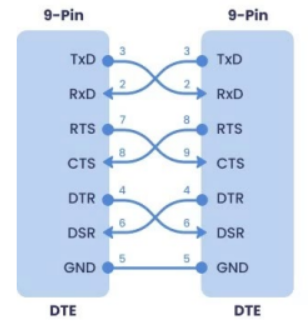
\includegraphics[width=0.8\textwidth]{assets/cap1/1.19.png}
\caption{Modelo DTE-DCE en una comunicación RS-232}
\label{fig:dte-dce}
\end{figure}

\subsection{Niveles de tensión: la gran diferencia con UART/TTL}

La diferencia más importante entre UART (a nivel TTL) y RS-232 es el \textbf{nivel de tensión}:

\begin{itemize}
    \item \textbf{UART/TTL} (0V / 3.3V o 5V): señales de bajo voltaje, idóneas para comunicaciones internas en PCB o cortas distancias.
    \item \textbf{RS-232} ($\pm$3V a $\pm$15V, típicamente $\pm$12V): señales de mayor amplitud, mucho más inmunes al ruido electromagnético y capaces de recorrer distancias mayores (hasta 15 metros a velocidades moderadas).
\end{itemize}

\begin{table}[htbp]
\centering
\small
\caption{Comparativa de niveles de tensión: TTL vs. RS-232}
\begin{tabular}{@{}lcc@{}}
\toprule
\textbf{Parámetro} & \textbf{UART/TTL} & \textbf{RS-232} \\
\midrule
Nivel lógico 0 (espacio) & 0V & +3V a +15V \\
Nivel lógico 1 (marca) & 3.3V o 5V & $-$3V a $-$15V \\
Inversión de señal & No & Sí (0 $\rightarrow$ +V, 1 $\rightarrow$ $-$V) \\
Distancia máxima & $<$1 metro & Hasta 15 metros \\
Inmunidad al ruido & Baja & Alta \\
\bottomrule
\end{tabular}
\end{table}

\textbf{¡Atención!} En RS-232, los niveles están \textbf{invertidos} respecto a TTL: un ``0'' lógico se transmite como voltaje positivo, y un ``1'' lógico como voltaje negativo. Esto es crucial al interpretar señales en un osciloscopio.

\subsection{Conectores y pines}

RS-232 utiliza conectores tipo D-sub:
\begin{itemize}
    \item \textbf{DB-9}: 9 pines, el más común hoy en día.
    \item \textbf{DB-25}: 25 pines, versión original del estándar.
\end{itemize}

De los 9 pines del DB-9, solo \textbf{tres} son imprescindibles para una comunicación básica:
\begin{enumerate}
    \item \textbf{TXD (Transmit Data, pin 3)}: salida de datos desde el DTE.
    \item \textbf{RXD (Receive Data, pin 2)}: entrada de datos al DTE.
    \item \textbf{GND (Signal Ground, pin 5)}: referencia de tierra común.
\end{enumerate}

Los pines restantes se usan para \textbf{control de flujo por hardware} (RTS, CTS, DTR, DSR, DCD, RI), aunque en muchas aplicaciones modernas se omiten.

\begin{figure}[H]
\centering
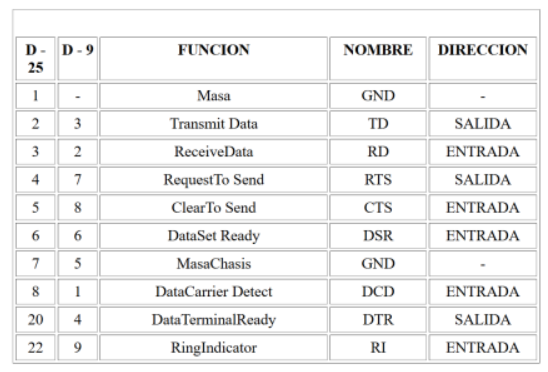
\includegraphics[width=0.8\textwidth]{assets/cap1/1.20.png}
\caption{Distribución de pines en un conector DB-9 para RS-232}
\label{fig:db9-pines}
\end{figure}

\subsection{Velocidad de subida y limitaciones}

El estándar RS-232 especifica una \textbf{velocidad de subida (slew rate)} máxima de $30\,$V/$\mu$s. Esta limitación intencionada evita que las transiciones rápidas generen interferencias electromagnéticas en señales adyacentes. Como consecuencia, la velocidad máxima de datos está limitada a aproximadamente \textbf{115.2 kb/s} (aunque en la práctica moderna se alcanzan 230.4 kb/s con cables cortos).

\subsection{Ventajas del RS-232 frente a otros protocolos}

\begin{itemize}
    \item \textbf{Mayor resistencia al ruido}: los voltajes de $\pm$12V son mucho más difíciles de alterar por interferencias que los 3.3V de TTL.
    \item \textbf{Distancias más largas}: hasta 15 metros frente a menos de 1 metro en TTL.
    \item \textbf{Compatibilidad universal}: existe hardware de conversión (TTL$\rightarrow$RS-232) muy económico y estandarizado.
    \item \textbf{Simplicidad de cableado}: solo dos hilos de datos + tierra para una comunicación básica.
\end{itemize}

\textbf{Limitaciones}: solo permite comunicación \textbf{punto a punto} (un DTE y un DCE), no es adecuado para redes multipunto. Para ello existen RS-485 y CAN bus.



\section{El protocolo USB: bus serie moderno}
\label{sec:usb}

\subsection{Introducción}

El \textbf{USB (Universal Serial Bus)} es el estándar de comunicación serie más extendido en la actualidad para la interconexión de periféricos con ordenadores y sistemas embebidos. Fue diseñado para sustituir a las interfaces antiguas (como RS-232, puerto paralelo y PS/2) con un único conector versátil, capaz de transmitir datos y alimentar el dispositivo al mismo tiempo.

\subsection{Características principales}

Las principales características del bus USB son:
\begin{itemize}
    \item \textbf{Topología punto a punto}: cada segmento conecta un host (o hub) con un único periférico o hub descendente.
    \item \textbf{Arquitectura maestro--esclavo}: el host (generalmente un PC) es el único maestro que inicia todas las comunicaciones; los periféricos responden únicamente cuando son interrogados.
    \item \textbf{Hasta 127 dispositivos}: mediante el uso de hubs en cascada, un único host puede gestionar hasta 127 periféricos simultáneamente.
    \item \textbf{Plug and Play}: los dispositivos pueden conectarse y desconectarse en caliente sin necesidad de apagar el equipo.
    \item \textbf{Alimentación integrada}: el cable proporciona una tensión nominal de 5\,V, lo que permite alimentar periféricos de bajo consumo directamente desde el bus.
    \item \textbf{Velocidades escalables}: desde 1.5\,Mb/s (Low Speed) hasta 20\,Gb/s (USB4) en sus versiones más recientes.
\end{itemize}

\subsection{Interfaz física y niveles eléctricos}

El cable USB estándar dispone de \textbf{cuatro hilos}:
\begin{enumerate}
    \item \textbf{VBUS} (+5\,V, rojo): alimentación para el periférico.
    \item \textbf{D--} (blanco): línea de datos diferencial negativa.
    \item \textbf{D+} (verde): línea de datos diferencial positiva.
    \item \textbf{GND} (negro): referencia de tierra común.
\end{enumerate}

La señal de datos se transmite por un \textbf{par trenzado diferencial} (D+ y D--) con una impedancia característica de 90\,$\Omega$. La sensibilidad del receptor es de al menos 200\,mV y debe soportar un alto factor de rechazo de modo común. La velocidad de transferencia puede ser de 1.5\,Mb/s, 12\,Mb/s, 480\,Mb/s, 5\,Gb/s, 10\,Gb/s o 20\,Gb/s, dependiendo de la versión del estándar.

\begin{figure}[H]
\centering
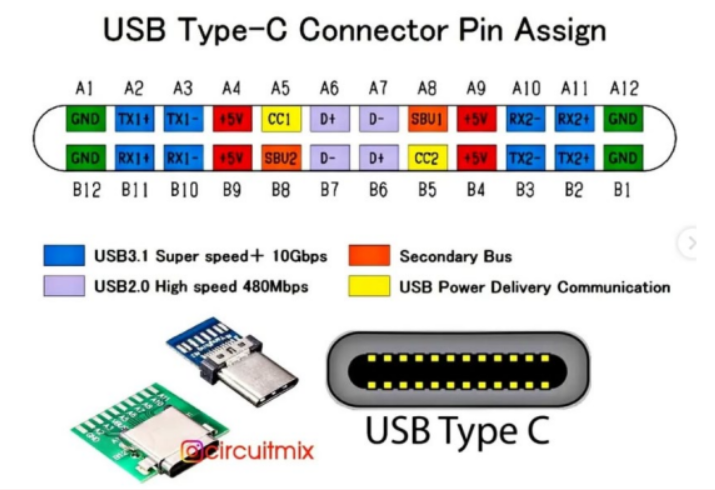
\includegraphics[width=0.8\textwidth]{assets/cap1/1.21.png}
\caption{Conector USB estándar y asignación de pines}
\label{fig:usb-pines}
\end{figure}

\subsection{Codificación y sincronización}

En USB, el reloj no se transmite por una línea separada, sino que se \textbf{recupera de los datos} mediante codificación NRZI. Para garantizar que haya suficientes transiciones y mantener la sincronización, el transmisor inserta \textbf{bits de relleno (bit stuffing)} cada vez que detecta seis unos consecutivos. Además, cada paquete comienza con un campo de sincronismo (SYNC) que permite al receptor ajustar su reloj interno.

\subsection{Terminología USB}

A continuación se definen los términos fundamentales que describen los elementos y roles de una arquitectura USB:

\begin{itemize}
    \item \textbf{Host.} Dispositivo maestro que inicia la comunicación (generalmente la computadora).
    \item \textbf{Hub.} Dispositivo que contiene uno o más conectores o conexiones internas hacia otros dispositivos USB, el cual habilita la comunicación entre el host y diversos dispositivos. Cada conector representa un puerto USB.
    \item \textbf{Dispositivo compuesto.} Es aquel dispositivo con múltiples interfaces independientes. Cada una tiene una dirección sobre el bus, pero cada interfaz puede tener un diferente driver de dispositivo en el host.
    \item \textbf{Puerto USB.} Cada host soporta solo un bus; cada conector en el bus representa un puerto USB. Por lo tanto, sobre el bus puede haber varios conectores, pero solo existe una ruta y solo un dispositivo puede transmitir información a un tiempo.
    \item \textbf{Driver.} Es un programa que habilita las aplicaciones para poder comunicarse con el dispositivo. Cada dispositivo sobre el bus debe tener un driver; algunos periféricos utilizan los drivers que trae el sistema operativo.
    \item \textbf{Puntos terminales (Endpoints).} Es una localidad específica dentro del dispositivo. El endpoint es un \textit{buffer} que almacena múltiples bytes, típicamente es un bloque de la memoria de datos o un registro dentro del microcontrolador. Todos los dispositivos deben soportar el punto terminal 0. Este punto terminal es el que recibe todo el control y las peticiones de estado durante la enumeración cuando el dispositivo está sobre el bus.
\end{itemize}

\begin{table}[htbp]
\centering
\small
\caption{Comparativa entre RS-232 y USB}
\begin{tabularx}{\textwidth}{@{}lXX@{}}
\toprule
\textbf{Característica} & \textbf{RS-232} & \textbf{USB} \\
\midrule
Modo de acceso & Punto a punto & Maestro--esclavo (host) \\
Balanceada & No (single-ended) & Sí (diferencial) \\
Velocidad máxima & 115.2\,kb/s & Hasta 20\,Gb/s (USB4) \\
Alimentación del bus & No & Sí (5\,V, hasta 500\,mA) \\
Conectores & DB-9, DB-25 & Tipo A, Tipo C, Micro-USB \\
Hot-plug & No & Sí \\
Número de dispositivos & 1 (P2P) & Hasta 127 (con hubs) \\
\bottomrule
\end{tabularx}
\end{table}


\section{Práctica 1: Comunicación UART con ESP32-S3}
\label{sec:practica1}

\subsection{Objetivos}

La Práctica 1 tiene como objetivos:
\begin{enumerate}
    \item Aprender a enviar y recibir datos mediante UART en modo asíncrono.
    \item Configurar el periférico UART de un microcontrolador (ESP32-S3) mediante su API.
    \item Examinar la señal UART física con un osciloscopio para comprender el formato de trama.
    \item Implementar una comunicación bidireccional entre un PC y un microcontrolador.
\end{enumerate}

\subsection{Material utilizado}

\begin{itemize}
    \item \textbf{Hardware}: PC, placa de desarrollo ESP32-S3-DevKitC-1, cable USB a TTL, osciloscopio.
    \item \textbf{Software}: Arduino IDE, Python (pyserial), drivers USB-UART.
\end{itemize}


\subsection{Marco teórico: protocolo UART}

\label{sec:uart}

Llegamos al protocolo protagonista de esta unidad y de la Práctica 1. El \textbf{UART} (Universal Asynchronous Receiver-Transmitter) es el protocolo de comunicación serie asíncrona más utilizado en electrónica digital y sistemas embebidos.

\subsubsection{Descripción del protocolo UART}

\begin{definicion}[formal de UART]
Un \textbf{UART (Universal Asynchronous Receiver-Transmitter)} es un circuito de hardware que implementa una comunicación serie asíncrona punto a punto, full-duplex, utilizando dos líneas de datos (TX y RX) y un nivel de tensión común de referencia (GND).
\end{definicion}

\textbf{Características principales}:
\begin{itemize}
    \item \textbf{Asíncrono}: no requiere línea de reloj compartida. La sincronización se logra mediante bits de inicio y parada.
    \item \textbf{Full-duplex}: ambos dispositivos pueden transmitir y recibir simultáneamente.
    \item \textbf{Punto a punto}: conecta exactamente dos dispositivos.
    \item \textbf{Pines mínimos}: TX (transmisión), RX (recepción) y GND (tierra común).
    \item \textbf{Niveles TTL}: típicamente 0V (lógica 0) y 3.3V o 5V (lógica 1). No confundir con RS-232, que usa voltajes mucho más altos ($\pm$12V).
\end{itemize}

\begin{figure}[H]
\centering
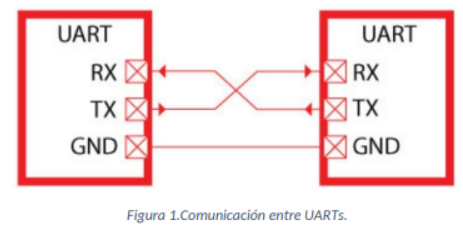
\includegraphics[width=0.8\textwidth]{assets/cap1/1.22.png}
\caption{Conexión cruzada entre dos dispositivos UART: TX de A con RX de B, y viceversa}
\label{fig:conexion-uart}
\end{figure}

\subsubsection{Formato de la trama UART}

La transmisión de un byte mediante UART sigue un formato estricto:

\begin{enumerate}
    \item \textbf{Estado de reposo (idle)}: la línea se mantiene a nivel alto (1) cuando no hay transmisión.
    \item \textbf{Bit de inicio (START)}: una transición a nivel bajo (0) durante un tiempo de bit. Indica al receptor que comienza un nuevo byte.
    \item \textbf{Bits de datos}: 5, 6, 7 u 8 bits (normalmente 8) que representan el carácter. El bit menos significativo (LSB) se envía primero.
    \item \textbf{Bit de paridad} (opcional): paridad par (E), impar (O), o sin paridad (N).
    \item \textbf{Bit(es) de parada (STOP)}: nivel alto (1) durante 0.5, 1, 1.5 o 2 tiempos de bit. Marca el final del byte.
\end{enumerate}

\begin{figure}[H]
\centering
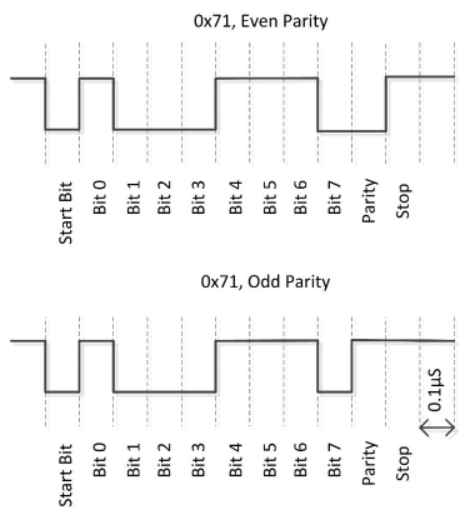
\includegraphics[width=0.8\textwidth]{assets/cap1/1.23.png}
\caption{Formato de trama UART para la configuración 8N1 (8 bits, sin paridad, 1 bit de parada)}
\label{fig:trama-uart}
\end{figure}

\subsubsection{Configuración de una comunicación UART}

Una comunicación UART se especifica mediante una cadena de parámetros:

\begin{center}
\textbf{\texttt{<velocidad> <bits de datos><paridad><bits de parada>}}
\end{center}

Ejemplos comunes:
\begin{itemize}
    \item \textbf{9600 8N1}: 9600 baudios, 8 bits de datos, sin paridad, 1 bit de parada.
    \item \textbf{115200 8E1}: 115200 baudios, 8 bits de datos, paridad par (Even), 1 bit de parada.
    \item \textbf{9600 8O1}: 9600 baudios, 8 bits de datos, paridad impar (Odd), 1 bit de parada.
\end{itemize}

\textbf{Velocidad de transmisión (baudios)}: indica el número de bits por segundo. Si el tiempo de bit es $T_b$, la velocidad en baudios es $1/T_b$. Por ejemplo, si $T_b = 0.1\,\mu$s, la velocidad es $10\,000\,000$ baudios (10 Mb/s).

\subsubsection{Control de flujo por hardware}

Cuando dos dispositivos tienen velocidades de procesamiento muy diferentes, el receptor puede no ser capaz de leer los datos tan rápido como el transmisor los envía. Para evitar la pérdida de información, se utiliza el \textbf{control de flujo por hardware} mediante dos señales adicionales:

\begin{itemize}
    \item \textbf{RTS (Request To Send)}: el transmisor activa esta señal para indicar que quiere enviar datos.
    \item \textbf{CTS (Clear To Send)}: el receptor activa esta señal para indicar que está listo para recibirlos.
\end{itemize}

El procedimiento es: Dispositivo A activa RTS → Dispositivo B responde con CTS → Dispositivo A transmite el byte → A desactiva RTS cuando termina → B desactiva CTS si no puede seguir.


\subsection{Configuración de pines UART en ESP32-S3}

El ESP32-S3 dispone de tres UARTs por hardware:

\begin{table}[htbp]
\centering
\small
\caption{Mapeo de pines UART en ESP32-S3}
\begin{tabular}{@{}lllll@{}}
\toprule
\textbf{UART} & \textbf{GPIO RX} & \textbf{GPIO TX} & \textbf{GPIO RTS} & \textbf{GPIO CTS} \\
\midrule
UART0 (Serial) & 44 & 43 & --- & --- \\
UART1 (Serial1) & 18 & 17 & 19 & 20 \\
UART2 (Serial2) & 16 & 15 & --- & --- \\
\bottomrule
\end{tabular}
\end{table}

\textbf{Nota importante}: UART0 está conectado internamente al conversor USB-UART de la propia placa, y se usa para programación y depuración (monitor serie del Arduino IDE). Para la comunicación con un PC externo o con otro dispositivo, se utiliza preferentemente UART1.

\subsection{Desarrollo de la práctica}

\subsubsection{Primera parte: envío de datos desde PC y desde ESP32}

Se desarrollaron dos versiones del programa:
\begin{enumerate}
    \item \textbf{Programa en Python (PC)}: abre el puerto COM asignado al cable USB-TTL con la velocidad configurada (ej. 9600 baudios) y envía un mensaje mediante \texttt{serial.write()}.
    \item \textbf{Programa en ESP32 (Arduino IDE)}: configura dos puertos serie:
    \begin{itemize}
        \item \texttt{Serial} → UART0 (USB interno), para depuración y monitor.
        \item \texttt{Serial1} → UART1 (GPIO 17 y 18), para la comunicación externa.
    \end{itemize}
\end{enumerate}

\begin{figure}[H]
\centering
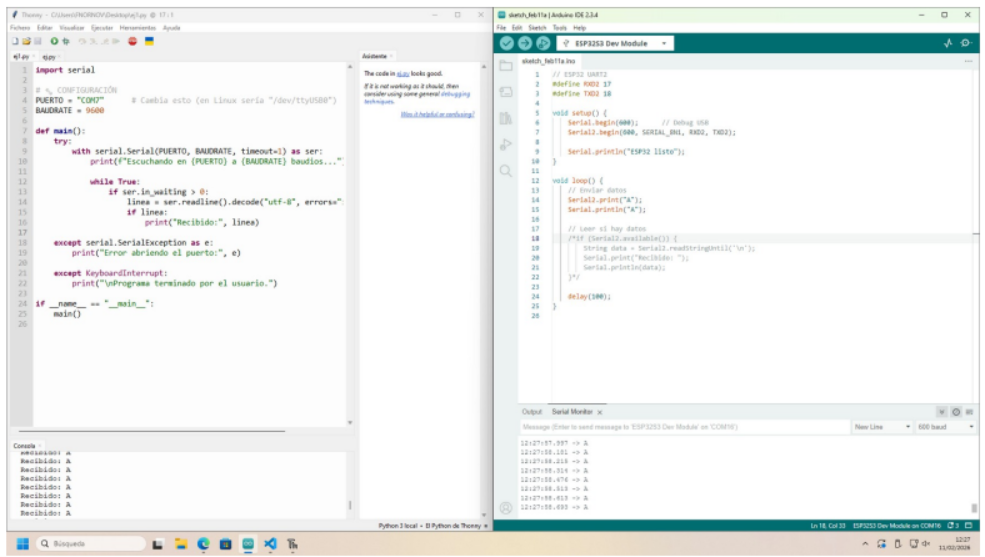
\includegraphics[width=0.8\textwidth]{assets/cap1/1.24.png}
\caption{Código de ejemplo para envío de datos por UART (PC o ESP32)}
\label{fig:codigo-envio}
\end{figure}

\subsubsection{Segunda parte: visualización con osciloscopio}

Se conectó la sonda del osciloscopio al pin TX (GPIO 18 o 17, según el caso) para observar la señal física. Enviando el carácter \texttt{'A'} (ASCII 0x41 = 01000001 en binario), se observó:

\begin{itemize}
    \item \textbf{Bit de inicio}: bajada de nivel (0 lógico).
    \item \textbf{Bits de datos}: \texttt{1} (LSB), \texttt{0}, \texttt{0}, \texttt{0}, \texttt{0}, \texttt{0}, \texttt{1}, \texttt{0} (MSB) — enviados en orden LSB primero, por lo que en la línea se lee \texttt{10000010} (bit0 a bit7).
    \item \textbf{Bit de parada}: retorno a nivel alto (1 lógico).
\end{itemize}

\begin{figure}[H]
\centering
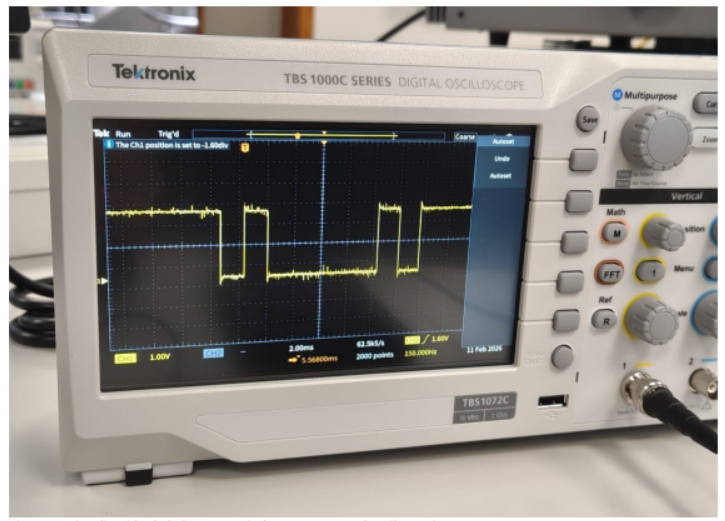
\includegraphics[width=0.8\textwidth]{assets/cap1/1.25.png}
\caption{Señal UART del carácter 'A' capturada en osciloscopio}
\label{fig:osciloscopio-a}
\end{figure}

\textbf{Decodificación manual}: la configuración utilizada fue 9600 8N1. Cada bit ocupa aproximadamente $1/9600 \approx 104\,\mu$s. En la pantalla del osciloscopio se puede medir la duración de cada pulso y confirmar que coincide con la velocidad configurada.

\subsubsection{Ampliación: comunicación bidireccional PC $\leftrightarrow$ ESP32}

Para la comunicación entre PC y ESP32 mediante el cable USB-TTL, se realizó el siguiente montaje:

\begin{itemize}
    \item Cable USB-TTL (verde = TX del cable) $\rightarrow$ GPIO 17 (RX de ESP32).
    \item GPIO 18 (TX de ESP32) $\rightarrow$ cable USB-TTL (blanco = RX del cable).
    \item GND común entre ambos dispositivos (esencial para la referencia de niveles).
\end{itemize}

\begin{figure}[H]
\centering
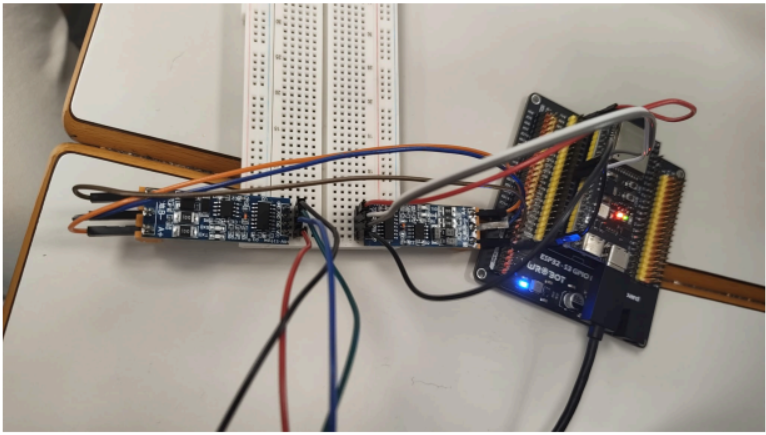
\includegraphics[width=0.8\textwidth]{assets/cap1/1.26.png}
\caption{Montaje físico para comunicación bidireccional PC $\leftrightarrow$ ESP32 por UART}
\label{fig:montaje-pc-esp32}
\end{figure}

\textbf{Problema detectado}: en una primera versión, se incluyó un carácter \texttt{\textbackslash n} (salto de línea) al final del mensaje. Esto generó una transición extra no deseada en la señal, visible en el osciloscopio. Al eliminarlo, la trama se ajustó exactamente al formato 8N1.

\textbf{Problema de buffer de recepción}: inicialmente, el código incluía una espera (delay) antes de leer. Esto causaba que varios bytes se acumularan en el buffer RX del ESP32 y se leyeran de golpe. Eliminando la espera, la lectura se hizo casi inmediata y se recibió correctamente un byte a la vez.

\subsection{Relación teoría-práctica}

\begin{table}[htbp]
\centering
\small
\caption{Conexión entre conceptos teóricos y elementos de la Práctica 1}
\begin{tabularx}{\textwidth}{@{}lX@{}}
\toprule
\textbf{Concepto teórico} & \textbf{Observación/aplicación en la práctica} \\
\midrule
Transmisión asíncrona & UART no usa reloj compartido; cada byte se sincroniza con su propio start bit \\
Formato de trama (start/stop) & Visualizado en osciloscopio: bajada (start), 8 bits, subida (stop) \\
Bit de paridad & Configuración 8N1: sin paridad; se podría cambiar a 8E1 o 8O1 \\
Velocidad (baudios) & 9600 baudios = $\sim$104\,$\mu$s por bit; medible en osciloscopio \\
Conexión P2P & Solo un PC y un ESP32; no es multidrop \\
Niveles TTL & ESP32 trabaja a 3.3V; el cable USB-TTL adapta a USB \\
Control de flujo (CTS/RTS) & GPIO 19 y 20 disponibles en ESP32, aunque no usados en esta práctica básica \\
Conexión cruzada TX$\leftrightarrow$RX & El TX del cable se conecta al RX del ESP32, y viceversa \\
\bottomrule
\end{tabularx}
\end{table}


\section{Práctica 2: Comunicación RS-232 entre ESP32-S3}
\label{sec:practica2}

\subsection{Objetivos}

La Práctica 2 amplía los conocimientos de la Práctica 1 introduciendo el estándar RS-232:
\begin{enumerate}
    \item Configurar la comunicación serie entre dos placas ESP32-S3 utilizando el protocolo RS-232.
    \item Observar las diferencias entre señales TTL (UART) y señales RS-232 (niveles de tensión e inversión).
    \item Verificar con osciloscopio la transmisión continua de un carácter y analizar su amplitud.
    \item Utilizar un cable \textbf{null-modem} para la comunicación directa entre dos DTE.
\end{enumerate}

\subsection{Material utilizado}

\begin{itemize}
    \item \textbf{Hardware}: 2 placas ESP32-S3-DevKitC-1, PC, 2 cables USB-TTL, 2 adaptadores TTL a RS-232, 2 adaptadores TTL a RS-485, cable null-modem, osciloscopio.
    \item \textbf{Software}: Arduino IDE.
\end{itemize}

\subsection{Desarrollo de la práctica}

\subsubsection{Primera parte: comunicación directa UART entre dos ESP32}

Se estableció una comunicación punto a punto entre dos placas ESP32-S3 mediante el puerto Serial2 (GPIO 16 y 17), conectando TX$\leftrightarrow$RX cruzado y GND común.

El código utilizado permite enviar o recibir simplemente comentando la parte no deseada:

\begin{lstlisting}[caption={Código ESP32 para transmisión/recepción por Serial2},label={lst:esp32-serial2}]
#define RXD2 17
#define TXD2 18

void setup() {
  Serial.begin(600);          // Debug USB
  Serial2.begin(600, SERIAL_8N1, RXD2, TXD2);
  Serial.println("ESP32 listo");
}

void loop() {
  // Enviar datos
  Serial2.print("S");
  Serial.println("S");
  
  // Leer si hay datos (comentar si solo se envia)
  /*if (Serial2.available()) {
    char data = Serial2.read('\n');
    Serial.print("Recibido: ");
    Serial.println(data);
  }*/
  
  delay(100);
}
\end{lstlisting}

\subsubsection{Segunda parte: verificación con osciloscopio}

Se conectó la sonda del osciloscopio al pin TX para verificar la transmisión continua del carácter \texttt{'S'} (ASCII 83 = 0x53 = \texttt{01010011} en binario).

\textbf{Análisis de la trama observada}:
\begin{itemize}
    \item El carácter \texttt{'S'} tiene valor binario: \texttt{01010011} (MSB $\rightarrow$ LSB).
    \item En UART, el \textbf{LSB se envía primero}, por lo que el orden de transmisión es: \texttt{11001010}.
    \item La trama completa es: \textbf{Start bit} (0) + \texttt{11001010} + \textbf{Stop bit} (1).
\end{itemize}

La señal observada en el osciloscopio coincidió exactamente con esta secuencia teórica.

\begin{figure}[H]
\centering
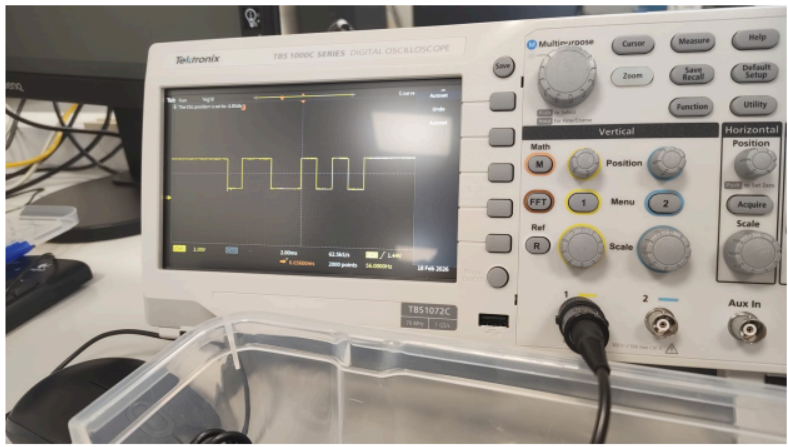
\includegraphics[width=0.8\textwidth]{assets/cap1/1.27.png}
\caption{Señal del carácter 'S' en osciloscopio (niveles TTL)}
\label{fig:osciloscopio-s}
\end{figure}

\subsubsection{Tercera parte: análisis de amplitud de la señal}

Se midieron los niveles de tensión de la señal TTL:

\begin{itemize}
    \item \textbf{Nivel alto}: aproximadamente $2.90\,\mathrm{V}$
    \item \textbf{Nivel bajo}: aproximadamente $0.70\,\mathrm{V}$
    \item \textbf{Amplitud pico a pico}: $\approx 2.20\,\mathrm{V}$
\end{itemize}

En condiciones ideales, una ESP32-S3 debería producir niveles de $0\,\mathrm{V}$ (bajo) y $3.3\,\mathrm{V}$ (alto). Las pequeñas desviaciones observadas se explican por:
\begin{itemize}
    \item Efecto de carga de la sonda del osciloscopio sobre el circuito.
    \item Caídas de tensión en el cableado.
    \item Referencia de masa no completamente estable.
    \item Ruido eléctrico ambiental, especialmente visible en los flancos.
\end{itemize}

\begin{figure}[H]
\centering
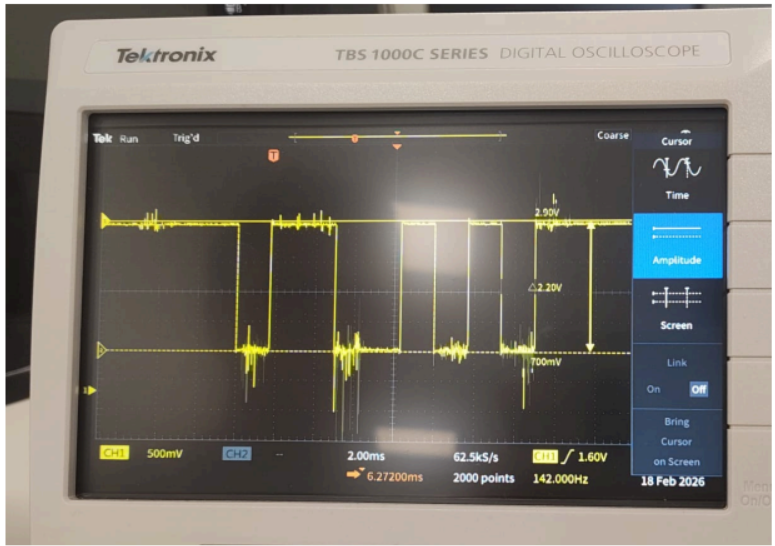
\includegraphics[width=0.8\textwidth]{assets/cap1/1.28.png}
\caption{Medida de amplitud de la señal TTL en osciloscopio}
\label{fig:amplitud-ttl}
\end{figure}

\subsubsection{Cuarta parte: uso del cable null-modem}

Un cable \textbf{null-modem} es un cable especial que cruza internamente las líneas TX y RX, permitiendo conectar dos equipos \textbf{DTE} (como dos ESP32) directamente sin necesidad de un DCE intermedio.

El montaje consiste en:
\begin{itemize}
    \item Conectar los adaptadores TTL$\rightarrow$RS-232 a cada ESP32.
    \item Unir ambos extremos mediante el cable null-modem.
    \item La conexión cruzada TX$\leftrightarrow$RX se realiza internamente en el cable.
\end{itemize}

Se comprobó que la comunicación funcionaba correctamente con el cable null-modem, y la señal observada en el osciloscopio coincidió con la obtenida anteriormente.

\begin{figure}[H]
\centering
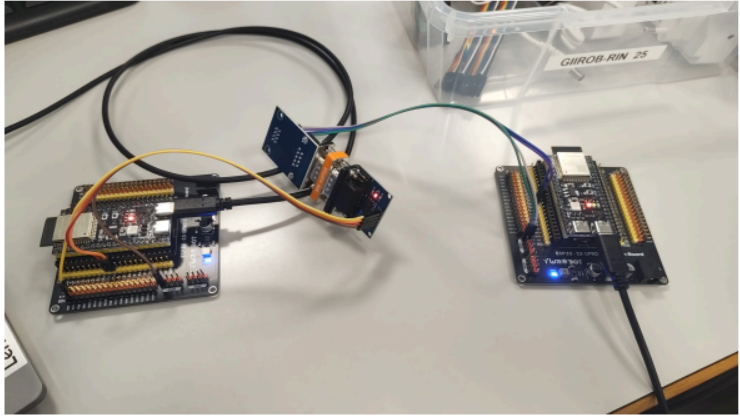
\includegraphics[width=0.8\textwidth]{assets/cap1/1.29.png}
\caption{Montaje con adaptadores TTL-RS-232 y cable null-modem}
\label{fig:null-modem}
\end{figure}

\subsection{Relación teoría-práctica: comparación UART vs. RS-232}

\begin{table}[htbp]
\centering
\small
\caption{Comparación entre Práctica 1 (UART/TTL) y Práctica 2 (RS-232)}
\begin{tabularx}{\textwidth}{@{}lXX@{}}
\toprule
\textbf{Aspecto} & \textbf{Práctica 1 (UART/TTL)} & \textbf{Práctica 2 (RS-232)} \\
\midrule
Nivel lógico 0 & 0V & $+$3V a $+$15V (típ. $+$12V) \\
Nivel lógico 1 & 3.3V & $-$3V a $-$15V (típ. $-$12V) \\
Inversión de señal & No & Sí \\
Distancia & $<$1 metro (USB-TTL) & Hasta 15 metros \\
Inmunidad al ruido & Baja & Alta \\
Hardware necesario & Cable USB-TTL & Adaptador TTL$\rightarrow$RS-232 \\
Conexión entre dos DTE & Cruzar TX-RX manualmente & Null-modem (cruce interno) \\
\bottomrule
\end{tabularx}
\end{table}


\section{Resumen de la Unidad 1}

\begin{itemize}
    \item Las \textbf{comunicaciones en serie} han sustituido a las paralelas en la mayoría de aplicaciones por su menor coste, mayor fiabilidad y capacidad para largas distancias.
    \item La \textbf{conexión diferencial} (balanceada) cancela el ruido común y es el estándar en entornos industriales.
    \item La \textbf{sincronización} puede ser asíncrona (UART), síncrona con reloj separado (SPI) o mediante recuperación desde los datos (CDR en USB/Ethernet).
    \item Los \textbf{protocolos} empaquetan los datos en tramas con delimitadores, direcciones y códigos de detección de errores.
    \item La \textbf{detección de errores} evoluciona desde el simple bit de paridad hasta el robusto CRC, pasando por el BCC.
    \item El \textbf{UART} es el protocolo asíncrono básico más usado en sistemas embebidos; su formato 8N1 es la configuración estándar.
    \item El estándar \textbf{RS-232} extiende el UART a niveles de tensión industriales ($\pm$12V), permitiendo distancias mayores y mayor inmunidad al ruido.
    \item La \textbf{Práctica 1} permite observar directamente la señal UART, confirmar el formato de trama, y establecer una comunicación real entre PC y microcontrolador.
    \item La \textbf{Práctica 2} demuestra la diferencia entre niveles TTL y RS-232, el uso de adaptadores, y la comunicación punto a punto entre dos microcontroladores.
\end{itemize}
